\subsubsection{Interfaces de Usuario}\label{Interfaces de Usuario}
A continuación se muestra la pantalla principal que será visible siempre que se inicie la aplicación, esta pantalla tiene 3 selectores (servidor, microcontrolador y nodo), por defecto mostrará los del primer nodo detectado. En la parte inferior vamos a poder observar la mejor marca de producción del día, y debajo de esta el estado de generación actual, es decir, el valor sensado cada 2 segundos. En la parte superior izquierda cuenta con una barra de navegación la cual nos permite acceder a otros componentes de la aplicación.  

\begin{figure}[H]
	\centering
	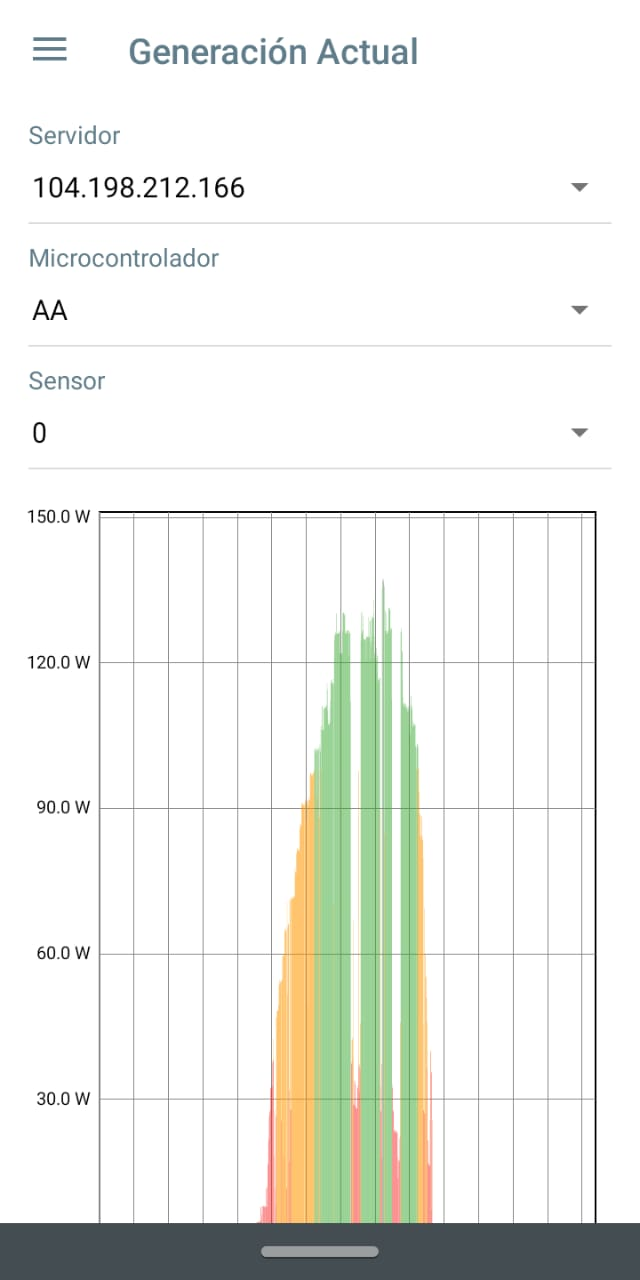
\includegraphics[scale=0.4]{Capitulo4/software/submodulos/images/man15.png}
	\caption{Interfaz de usuario Ver Generación Actual}
	\label{fig:monitoreoReal}
\end{figure}

\begin{figure}[H]
	\centering
	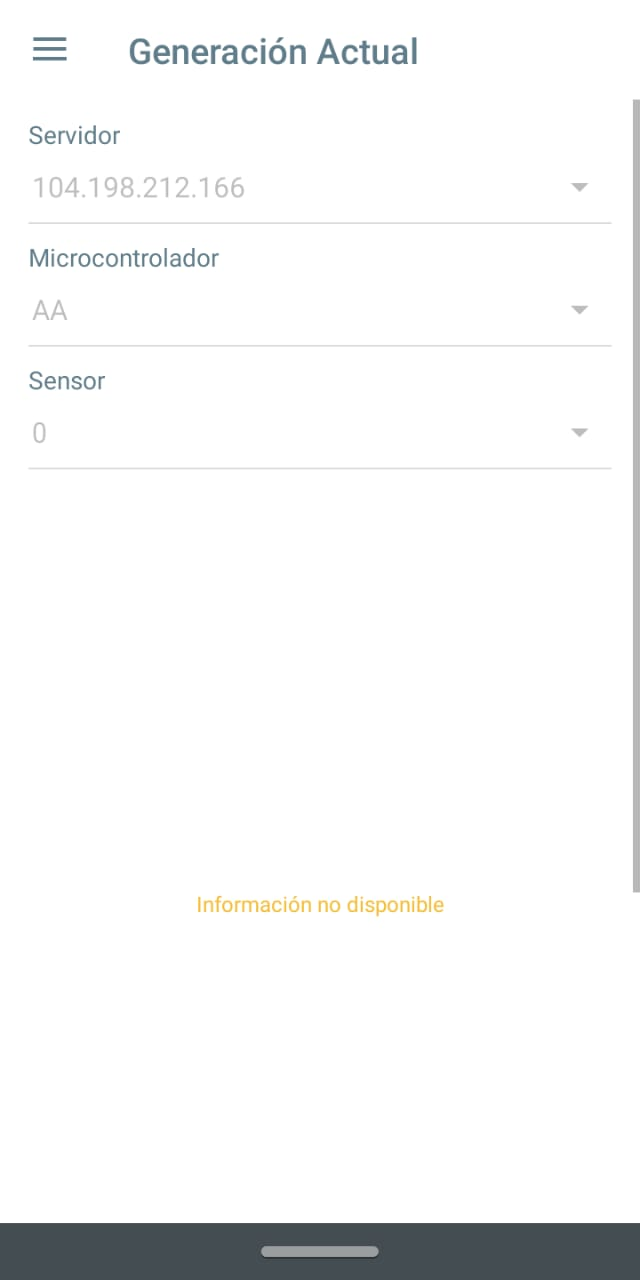
\includegraphics[scale=0.4]{Capitulo4/software/submodulos/images/man1.png}
	\caption{Interfaz de usuario Ejemplo de opciones de selección de sensor}
	\label{fig:monitoreo}
\end{figure}

La pantalla mostrada a continuación contiene las 4 posibles opciones que tiene la barra de navegación de la pantalla principal \ref{fig:monitoreo}, cada uno de los 4 botones nos redirige a un componente de la aplicación.

\begin{figure}[H]
	\centering
	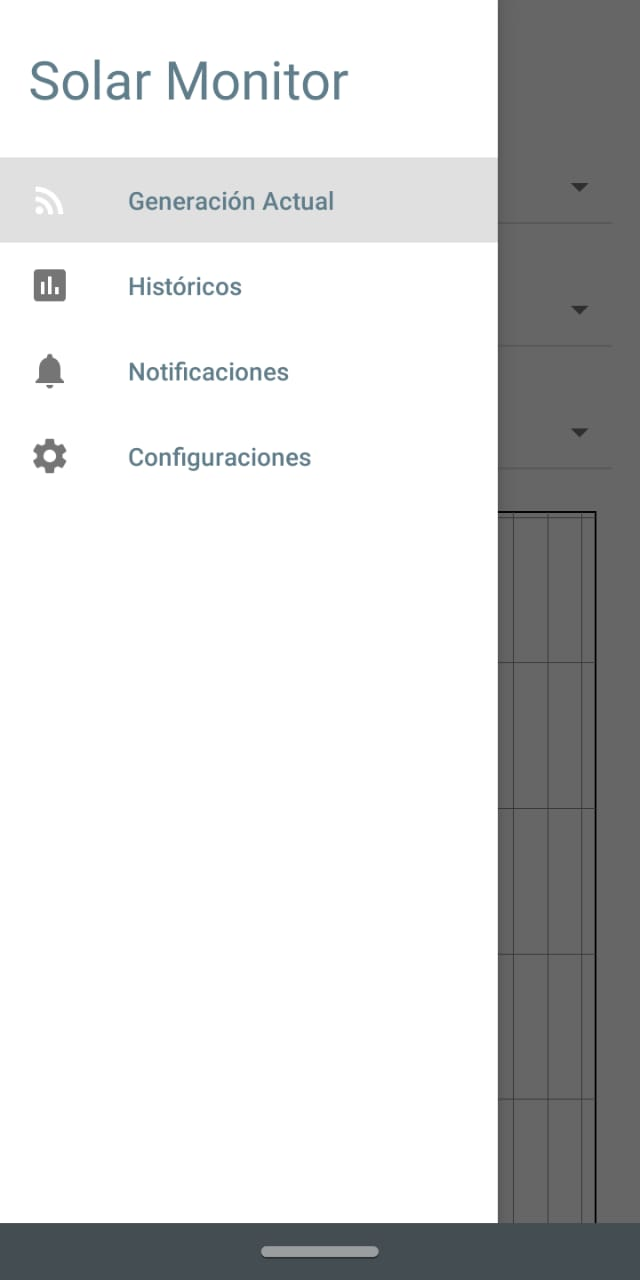
\includegraphics[scale=0.4]{Capitulo4/software/submodulos/images/man2.png}
	\caption{Interfaz de usuario Barra de Navegación}
	\label{fig:Barra de navegacion}
\end{figure}

En la siguiente pantalla podemos observar la pantalla de históricos (opción disponible en la barra de navegación de la pantalla \ref{fig:Barra de navegacion}), la cual por defecto siempre que sea accedida mostrará la gráfica de generación semanal y con el primer o único sensor. La pantalla posee 5 distintos selectores, el primero permite elegir el servidor, el segundo el microcontrolador, el tercero el sensor, el cuarto el periodo y en caso de que el periodo sea ''Año'' se habilitará el quinto, para así poder elegir un año en específico, de lo contrario permanecerá deshabilitado.

\begin{figure}[H]
	\centering
	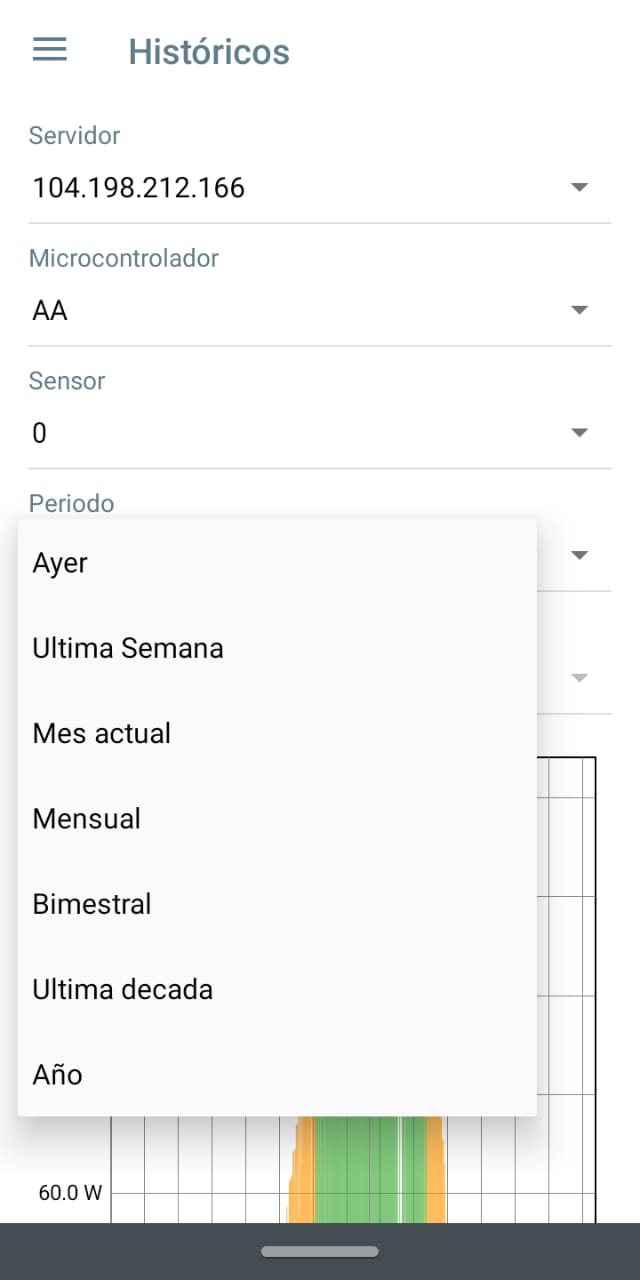
\includegraphics[scale=0.4]{Capitulo4/software/submodulos/images/man34.png}
	\caption{Interfaz de usuario Opciones de Intervalo}
	\label{fig:Opciones de Intervalo}
\end{figure}

La siguientes pantallas muestran los distintos periodos en los que se puede generar una gráfica de barras que representa datos históricos, la figura \ref{fig:Historico ayer} grafica las muestras del día de ayer, la figura \ref{fig:Historico semanal} grafica las muestras de la última semana, la figura \ref{fig:Historico mes actual} grafica las muestras de los días del mes actual, la figura \ref{fig:Historico mensual} grafica las muestras de los meses del año en curso, la figura \ref{fig:Historico bimestral} grafica las muestras de bimestrales del año en curso, la figura \ref{fig:Historico ultima decada} grafica las muestras de los últimos 10 años y la figura \ref{fig:Historico anual} grafica las muestras de los 12 meses de el año seleccionado.

\begin{figure}[H]
	\centering
	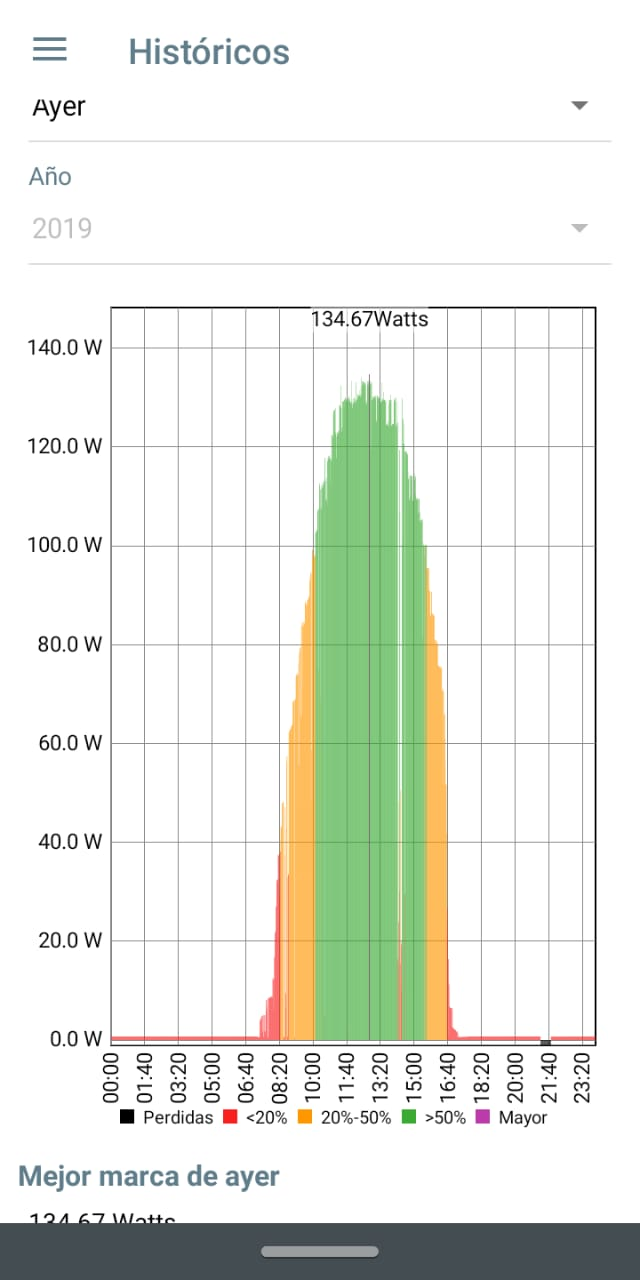
\includegraphics[scale=0.4]{Capitulo4/software/submodulos/images/man25.png}
	\caption{Interfaz de usuario Histórico de ayer}
	\label{fig:Historico ayer}
\end{figure}

\begin{figure}[H]
	\centering
	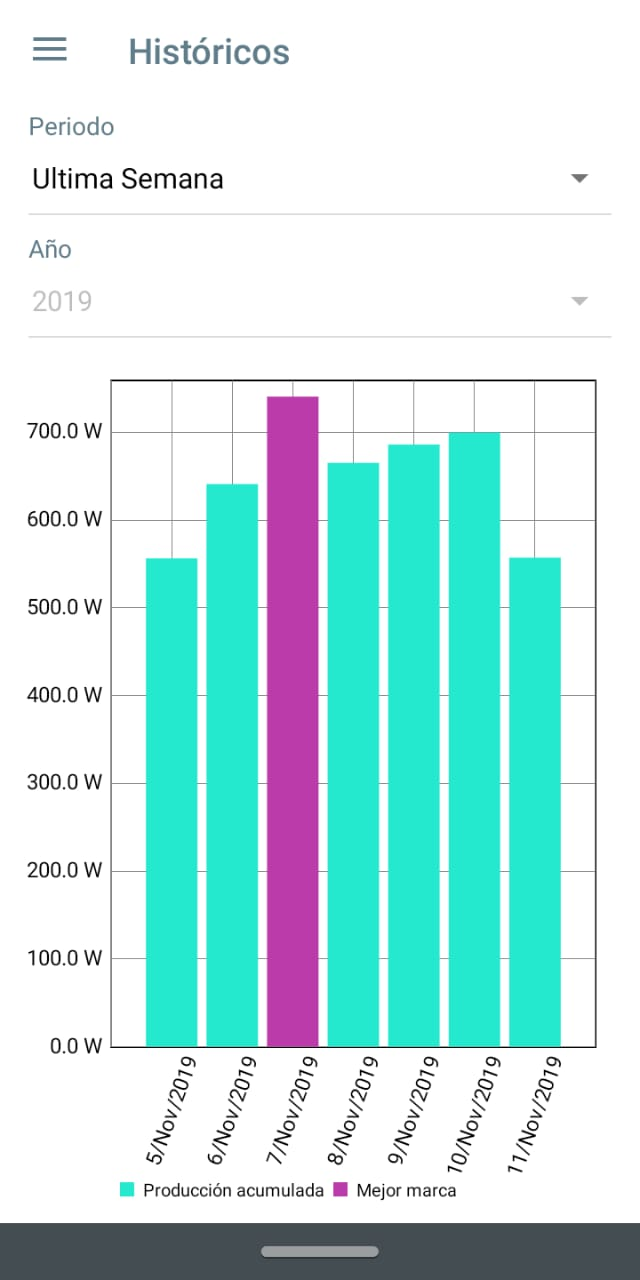
\includegraphics[scale=0.4]{Capitulo4/software/submodulos/images/man26.png}
	\caption{Interfaz de usuario Histórico semanal}
	\label{fig:Historico semanal}
\end{figure}

\begin{figure}[H]
	\centering
	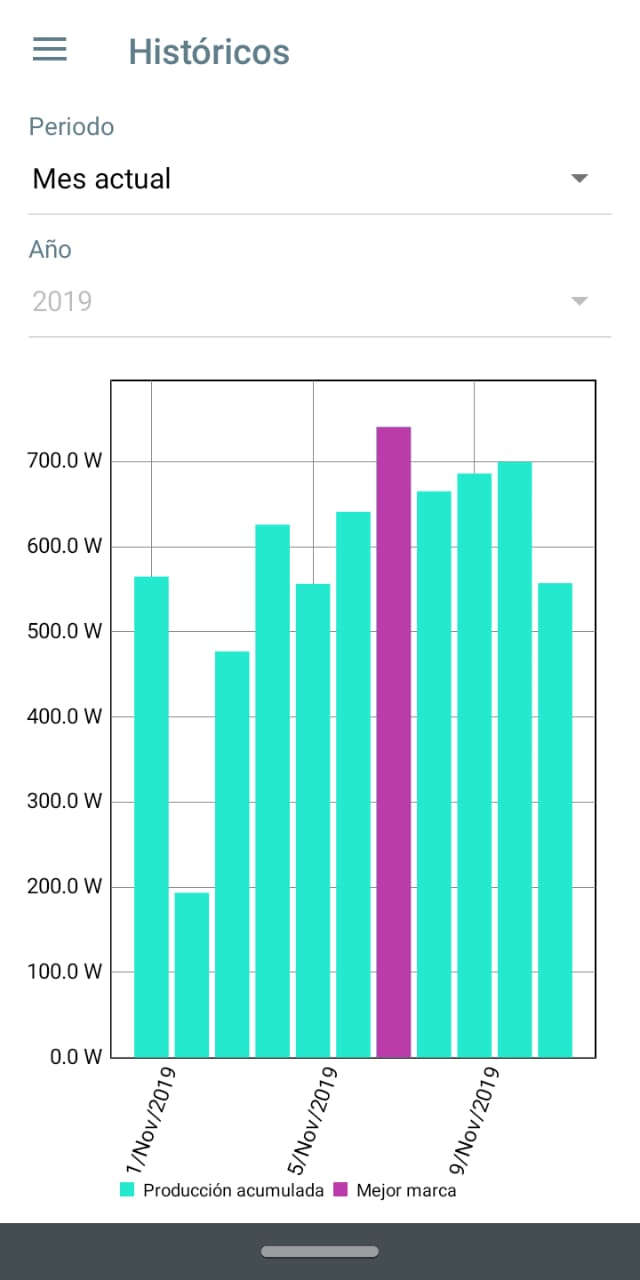
\includegraphics[scale=0.4]{Capitulo4/software/submodulos/images/man27.png}
	\caption{Interfaz de usuario Histórico del mes actual}
	\label{fig:Historico mes actual}
\end{figure}

\begin{figure}[H]
	\centering
	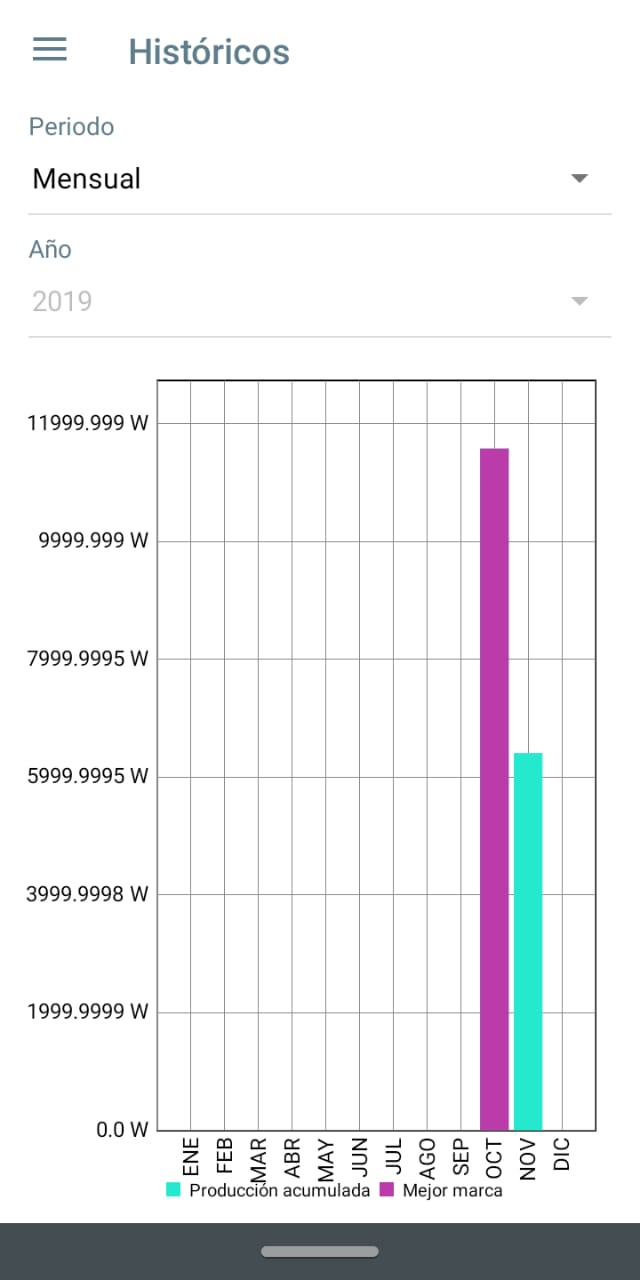
\includegraphics[scale=0.4]{Capitulo4/software/submodulos/images/man28.png}
	\caption{Interfaz de usuario Histórico mensual}
	\label{fig:Historico mensual}
\end{figure}

\begin{figure}[H]
	\centering
	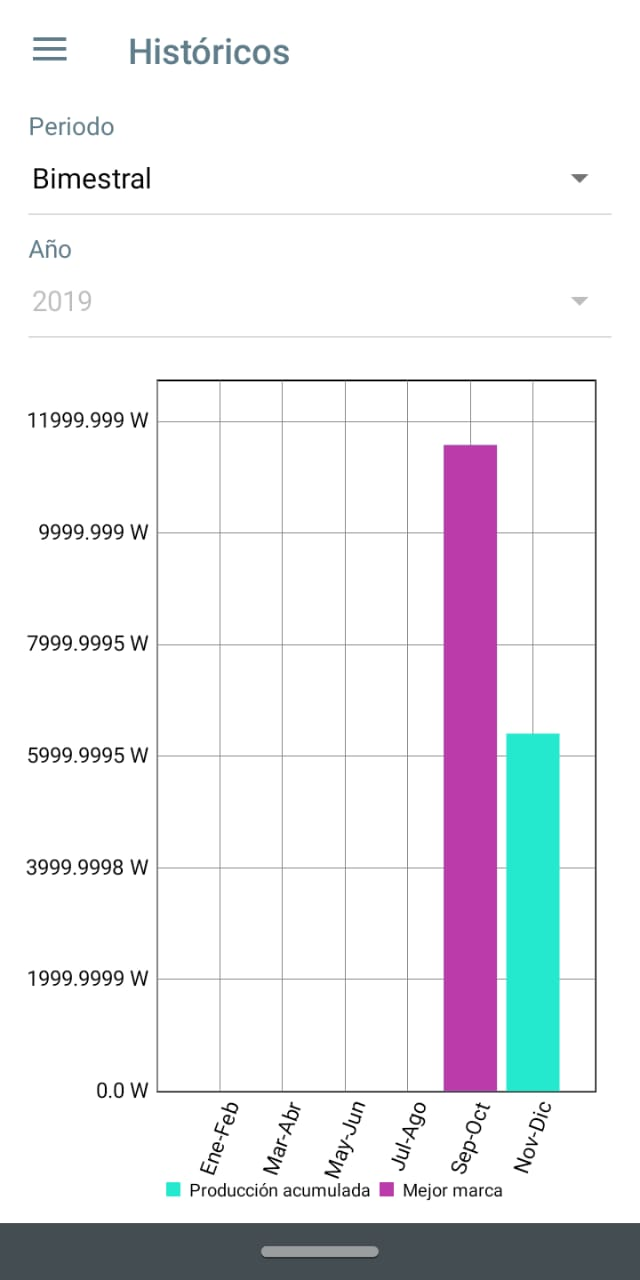
\includegraphics[scale=0.4]{Capitulo4/software/submodulos/images/man29.png}
	\caption{Interfaz de usuario Histórico bimestral}
	\label{fig:Historico bimestral}
\end{figure}

\begin{figure}[H]
	\centering
	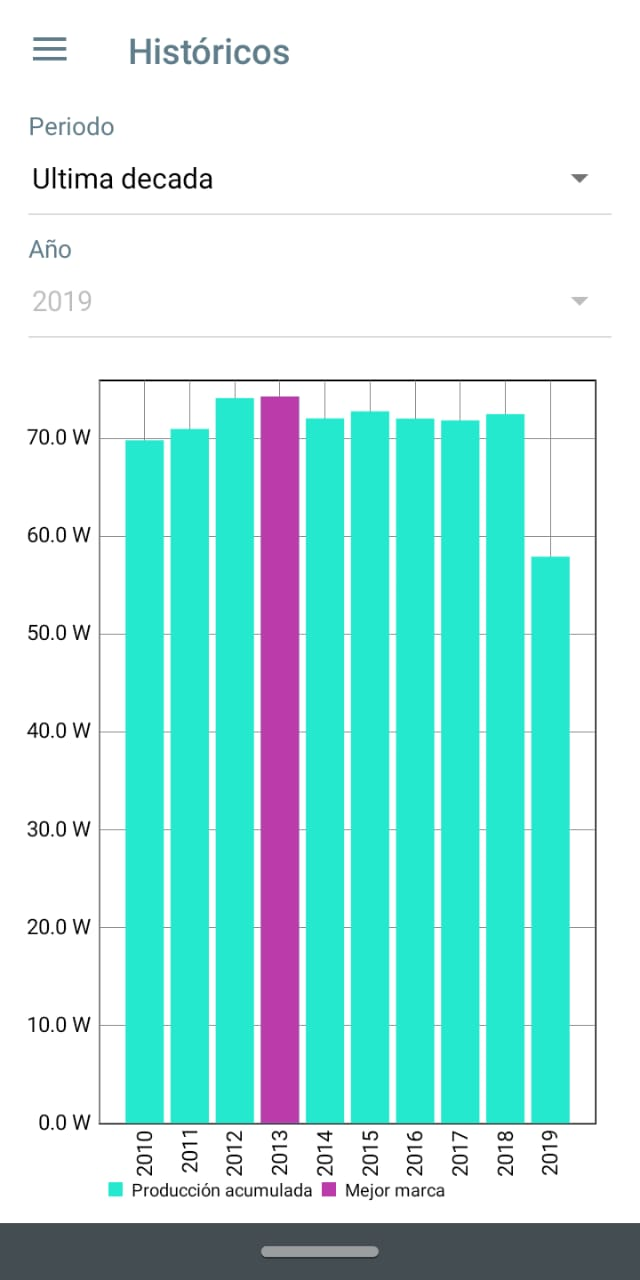
\includegraphics[scale=0.4]{Capitulo4/software/submodulos/images/man30.png}
	\caption{Interfaz de usuario Histórico de última década}
	\label{fig:Historico ultima decada}
\end{figure}

\begin{figure}[H]
	\centering
	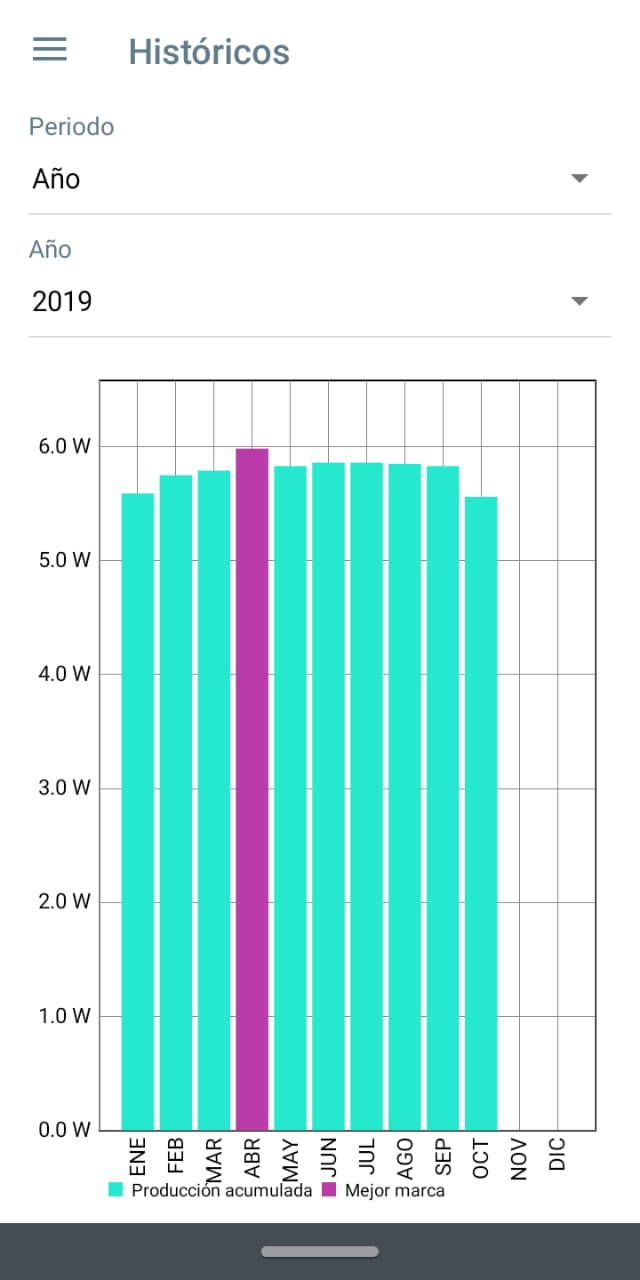
\includegraphics[scale=0.4]{Capitulo4/software/submodulos/images/man31.png}
	\caption{Interfaz de usuario Histórico anual}
	\label{fig:Historico anual}
\end{figure}

La pantalla de configuraciones permite al usuario habilitar o deshabilitar el servicio de notificaciones, añadir nuevos servidores y enlistar los servidores que han sido almacenados.

\begin{figure}[H]
	\centering
	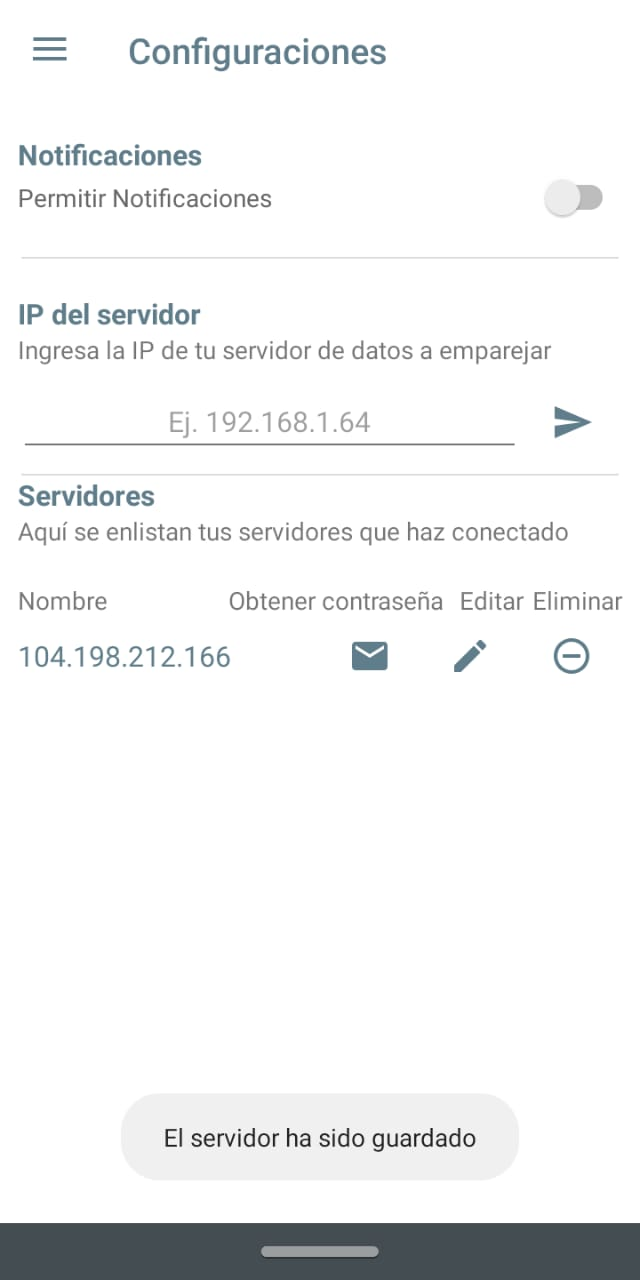
\includegraphics[scale=0.4]{Capitulo4/software/submodulos/images/man6.png}
	\caption{Interfaz de usuario Configuraciones}
	\label{fig:Configuraciones}
\end{figure}

Las siguientes pantallas aparecerán cuando el usuario desea agregar un nuevo servidor para monitorear los nodos. 
\begin{figure}[H]
	\centering
	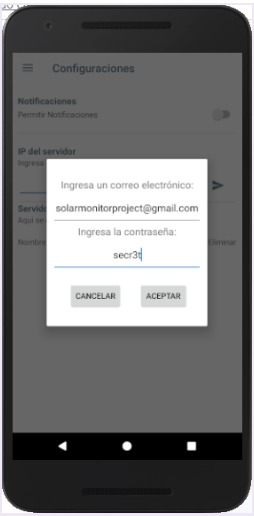
\includegraphics[scale=0.8]{Capitulo4/software/submodulos/images/man37.png}
	\caption{Interfaz de usuario Ingresar correo y contraseña}
	\label{fig:Correo y contrasena}
\end{figure}

\begin{figure}[H]
	\centering
	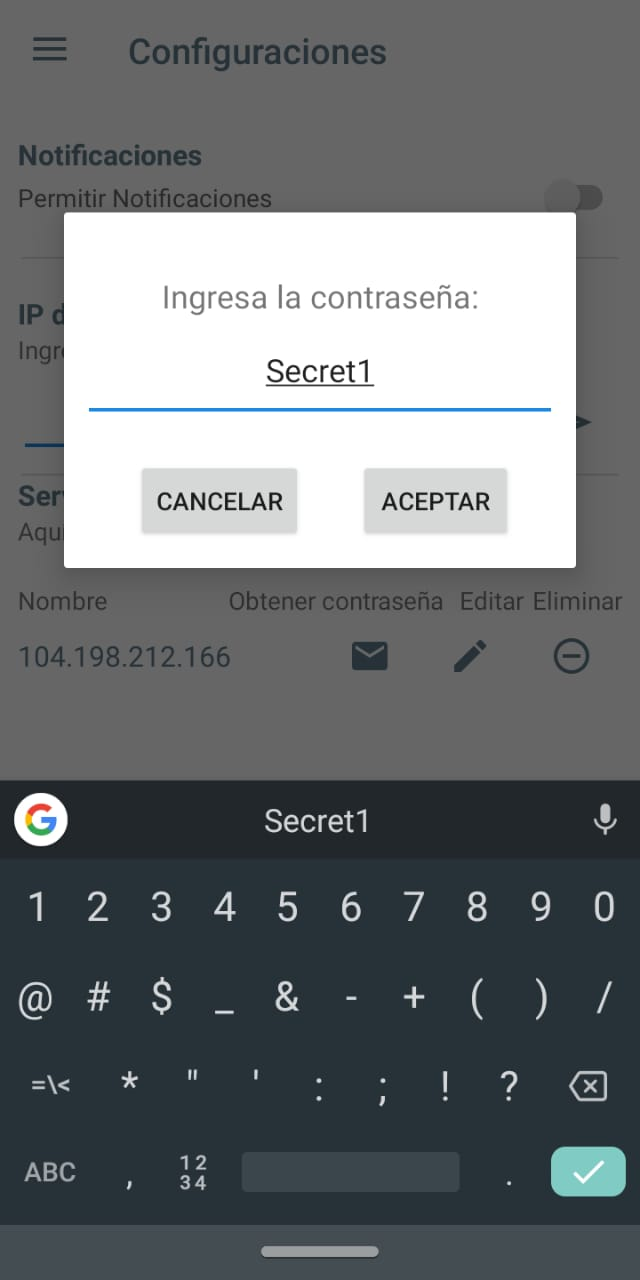
\includegraphics[scale=0.4]{Capitulo4/software/submodulos/images/man10.png}
	\caption{Interfaz de usuario Ingresar contraseña}
	\label{fig:contrasena}
\end{figure}

Cuando el usuario agrega un servidor a la aplicación, se va a mostrar en la lista de servidores y tendrá las opciones que le permiten: recuperar la contraseña por medio de correo electrónico, editar el nombre del servidor o bien eliminarlo.

\begin{figure}[H]
	\centering
	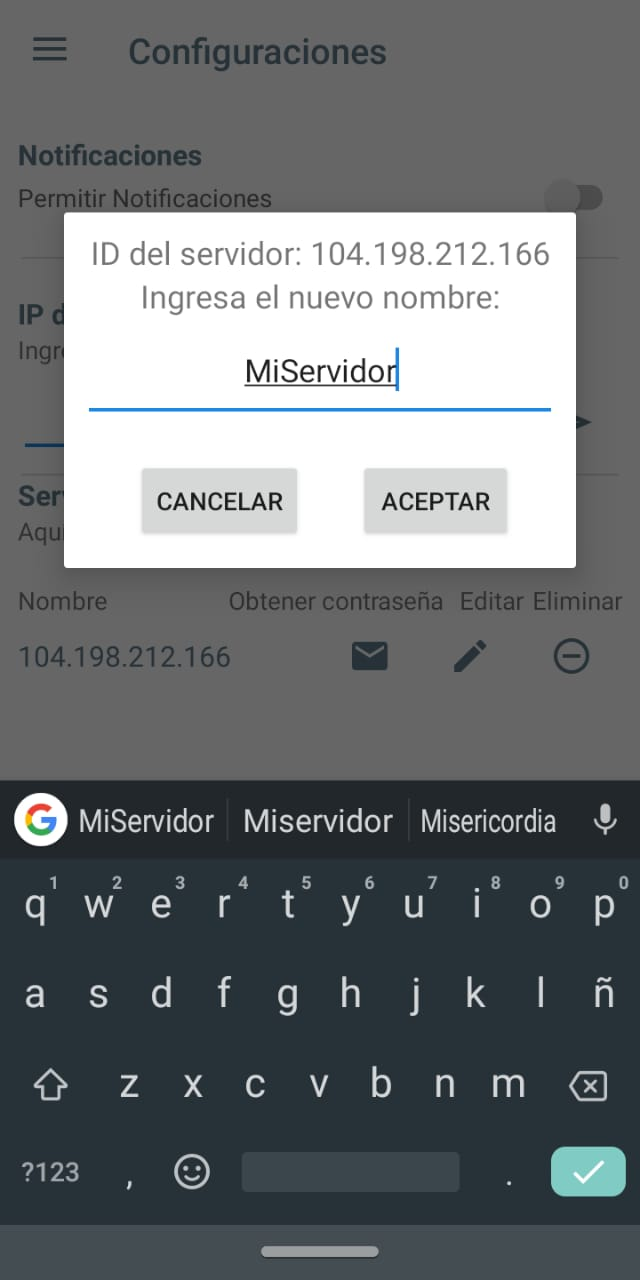
\includegraphics[scale=0.4]{Capitulo4/software/submodulos/images/man12.png}
	\caption{Interfaz de usuario Editar nombre de servidor}
	\label{fig:Editar servidor}
\end{figure}

\begin{figure}[H]
	\centering
	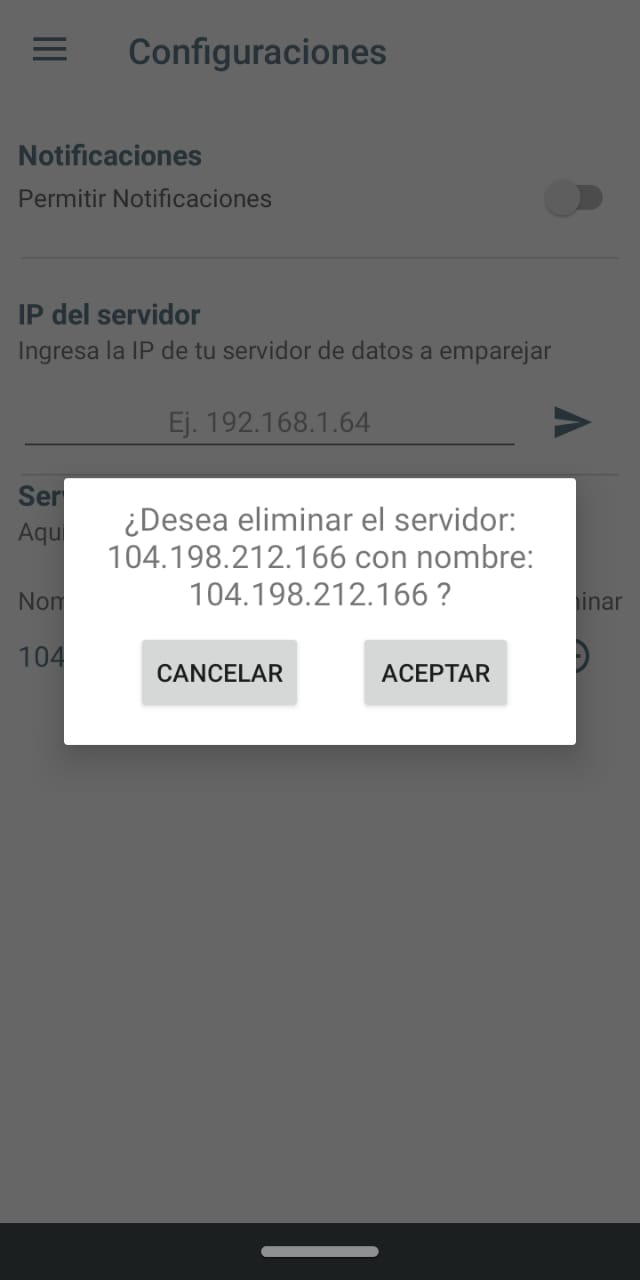
\includegraphics[scale=0.4]{Capitulo4/software/submodulos/images/man35.png}
	\caption{Interfaz de usuario Eliminar servidor}
	\label{fig:Eliminar servidor}
\end{figure}

La pantalla siguiente muestra una lista con las notificaciones que han sido almacenadas durante el proceso de monitoreo, es decir, cuando el usuario habilita el servicio en segundo plano.

\begin{figure}[H]
	\centering
	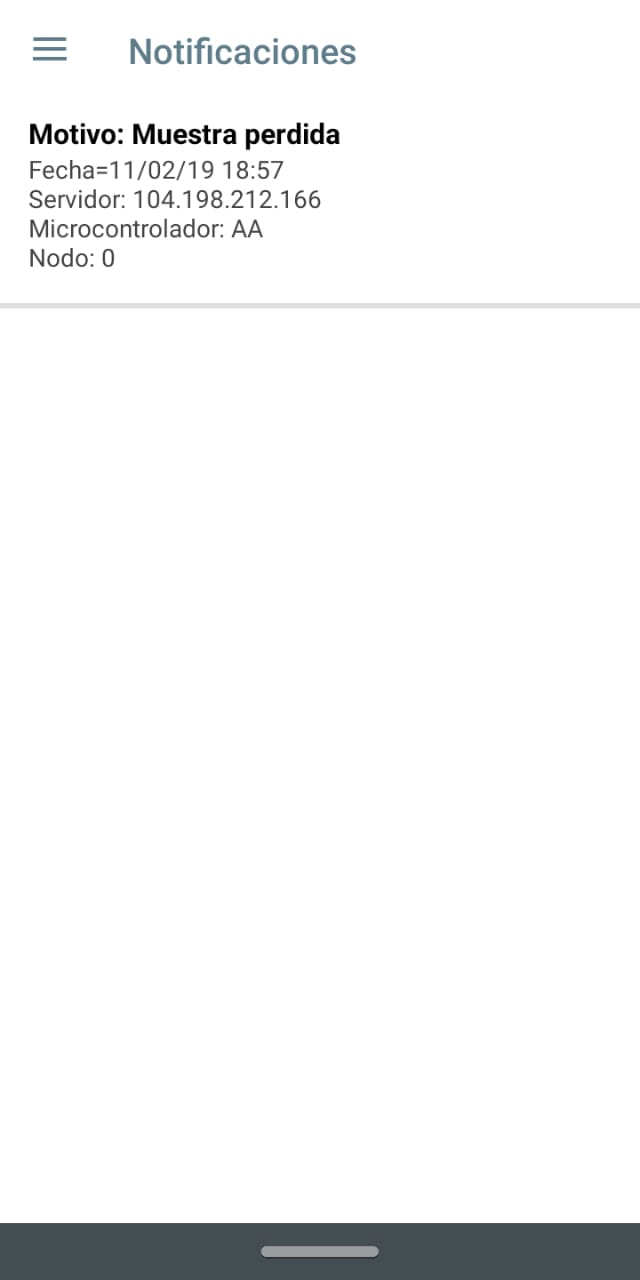
\includegraphics[scale=0.4]{Capitulo4/software/submodulos/images/man22.png}
	\caption{Interfaz de usuario Lista de Notificaciones}
	\label{fig:Lista de Notificaciones}
\end{figure}


\subsubsection{Notificaciones}\label{Notificaciones}
Cuando ocurra un suceso que amerite realizar una notificación como ha sido detallado en capítulos anteriores, se creará una notificación a nivel de Android, la cual mostrará la causa de la notificación.

\begin{figure}[H]
	\centering
	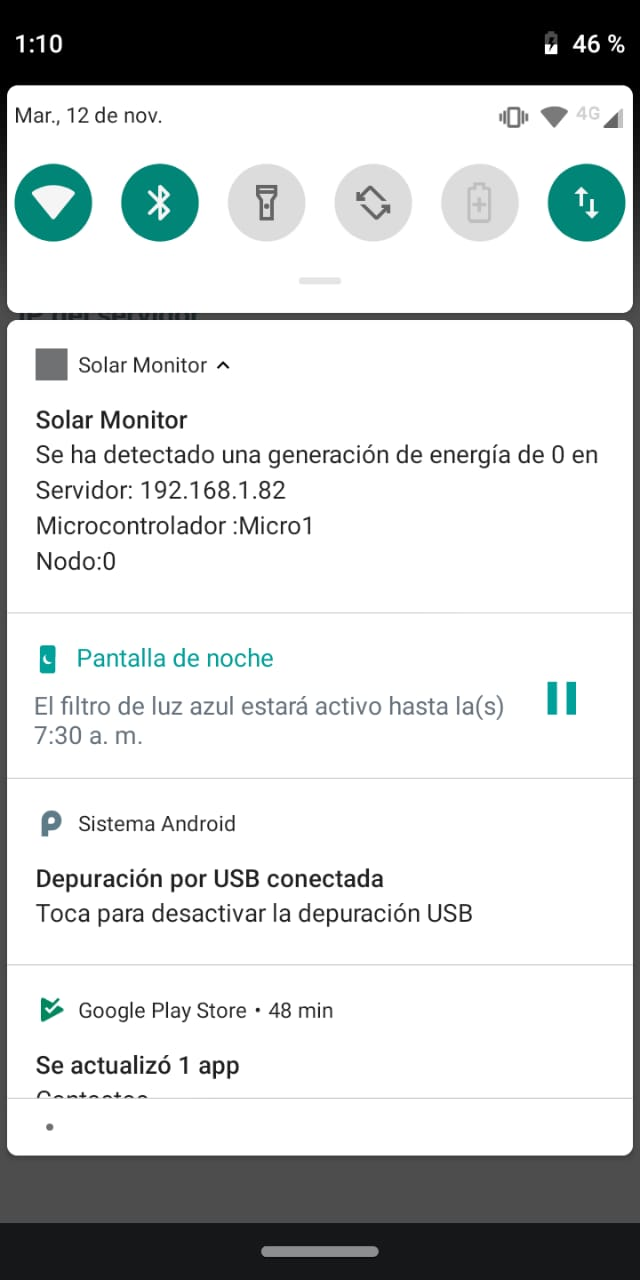
\includegraphics[scale=0.4]{Capitulo4/software/submodulos/images/man36.png}
	\caption{Ejemplo de Notificación (Generación de energía de 0)}
	\label{fig:Ejemplo de notificacion}
\end{figure}
